% THIS IS SIGPROC-SP.TEX - VERSION 3.1
% WORKS WITH V3.2SP OF ACM_PROC_ARTICLE-SP.CLS
% APRIL 2009
% For tracking purposes - this is V3.1SP - APRIL 2009

\documentclass{acm_proc_article-sp}

\usepackage[utf8]{inputenc}
\usepackage[english]{babel} % English language/hyphenation
\usepackage{booktabs}
%\usepackage{multicol}
\newcommand{\ra}[1]{\renewcommand{\arraystretch}{#1}}
\usepackage{float}
\usepackage{enumitem}

% bib
\usepackage[autostyle]{csquotes}
\usepackage[
  backend=biber,
  style=numeric-comp,
  natbib=true,
  url=false,
  doi=true,
]{biblatex}
\addbibresource{ref.bib}

\begin{document}
%\begin{multicols}{2}

\title
{
	Sequence Labeling for Gait Analysis using LSTM
    %Automated Event Detection from Kinematic Data of Human Walking
}
%
% You need the command \numberofauthors to handle the 'placement
% and alignment' of the authors beneath the title.
%
% For aesthetic reasons, we recommend 'three authors at a time'
% i.e. three 'name/affiliation blocks' be placed beneath the title.
%
% NOTE: You are NOT restricted in how many 'rows' of
% "name/affiliations" may appear. We just ask that you restrict
% the number of 'columns' to three.
%
% Because of the available 'opening page real-estate'
% we ask you to refrain from putting more than six authors
% (two rows with three columns) beneath the article title.
% More than six makes the first-page appear very cluttered indeed.
%
% Use the \alignauthor commands to handle the names
% and affiliations for an 'aesthetic maximum' of six authors.
% Add names, affiliations, addresses for
% the seventh etc. author(s) as the argument for the
% \additionalauthors command.
% These 'additional authors' will be output/set for you
% without further effort on your part as the last section in
% the body of your article BEFORE References or any Appendices.

\numberofauthors{3} %  in this sample file, there are a *total*
% of EIGHT authors. SIX appear on the 'first-page' (for formatting
% reasons) and the remaining two appear in the \additionalauthors section.
%
\author{
% You can go ahead and credit any number of authors here,
% e.g. one 'row of three' or two rows (consisting of one row of three
% and a second row of one, two or three).
%
% The command \alignauthor (no curly braces needed) should
% precede each author name, affiliation/snail-mail address and
% e-mail address. Additionally, tag each line of
% affiliation/address with \affaddr, and tag the
% e-mail address with \email.
%
% 1st. author
\alignauthor
Pablo A. Iturralde\\ 
	   \affaddr{Bioengineering Department}\\        
       \affaddr{University of Pittsburgh}\\
       \affaddr{Pittsburgh,PA}\\
       \email{pai7@pitt.edu}
% 2nd. author
\alignauthor
Yin Zhong\\
       \affaddr{The Robotics Institute}\\
       \affaddr{Carnegie Mellon University}\\
       \affaddr{Pittsburgh,PA}\\
       \email{yinzhong@andrew.cmu.edu}
\and  % use '\and' if you need 'another row' of author names
% 3rd. author
\alignauthor Jakob Bauer\\
       \affaddr{School of Computer Science}\\
       \affaddr{Carnegie Mellon University}\\
       \affaddr{Pittsburgh,PA}\\
       \email{jsbauer@andrew.cmu.edu}
}
       
\maketitle

\section{Data}
For the initial training purposes, we selected data from 8 healthy subjects walking in a treadmill at three different speeds for 100 seconds each. Additionally, we took data from 13 stroke subjects, walking at a single speed for 100 seconds. For each subject, the input data is 3D marker position of 18 different markers placed in the same anatomical positions for each subject, sampled at 100Hz. The event labels (target) were computed from ground force reaction data samples at 1kHz for healthy subjects, and 2kHz for stroke subjects. This is currently considered the gold standard \cite{miller_gait_2009,miller_gait_2009,Hreljac2000}. \\
%The problem is then to classify each sample in time as one of four different classes: both feet in contact with the ground, both feet off the ground, left feet only on the ground and right feet only on the ground. 
\section{Algorithms}

In order to compare our results, we implemented two algorithms presented in the literature: a heuristic-based method \cite{oconnor_automatic_2007}, and a neural-network approach \cite{miller_gait_2009}.

\subsection{O'Connor's Heuristic}
\citet{oconnor_automatic_2007} describe a heuristic to compute gait events by just considering vertical and horizontal speed of heel and toe markers respectively, and using a peak detection algorithm.

\subsection{Miller's Neural Network}
\citet{miller_gait_2009} is one of the few data-driven efforts of event estimation. It uses a classical NN to classify each sample. The inputs are computed from the position, instantaneous velocity and instantaneous acceleration of each available motion-capture marker in a time-window centered around the desired time sample. Because the inputs are too many (the total input size grows linearly with the window size and the number of markers), a dimensionality reduction technique (PCA) is used before training the NN.

\subsection{Our approach: Long Short Term Memory Neural Network}
%\vspace{-1cm}

Gait event detection is a form of \textit{sequence labeling}, i.e., assigning a sequence of labels to a sequence of data.
One approach to sequence labeling is the use of recurrent neural networks (RNN). However, due to the vanishing gradient problem RNNs cannot store information for a long time which means that their usefulness for sequence labeling is limited.
One solution to this problem is the use of a Long Short-Term Memory (LSTM) architecture instead of conventional RNNs \cite{graves_supervised_2012}.
In LSTM, the summation units in the hidden layer are replaced with so-called memory blocks.
These blocks consist of a memory cell as well as three multiplicative units called input gate, output gate and forget gate.
The gates allow information to be stored in the memory cell for long periods of time.
While we haven't decided on the overall design of our LSTM network yet, it will probably have specifications along the lines of:
\begin{itemize}[noitemsep,nolistsep]
\item Up to 54 input units that each take the sequence corresponding to one marker as input; the reason we might not need all 54 marker sequences is that some of the markers (e.g., for the hip) presumably carry little useful information.
\item A hidden layer of LSTM memory blocks; the exact number will depend on the number of input units.
\item 2 output units (one for each leg); the output will be thresholded with '0' corresponding to stance phase and '1' corresponding to swing phase.
\end{itemize}

\section{Computational Resources}

For the LSTM network we are using
an Amazon EC2 instance of type g2.2xlarge.
This instance type comes with an 8 core 2.6 GHz Intel Xeon E5-2670 processor and an Nvidia GRID K520 GPU that is composed of two 4 GB GK104 GPUs.
We chose Torch as our computing framework.

\section{Intermediate Results}
We implemented and tested the two methods described in \cite{oconnor_automatic_2007} and \cite{miller_gait_2009}. Results are in line with the ones presented on each paper. Summaries of the true error (detected event time minus actual event time) can be found in Figures~\ref{fig:oconner} and \ref{fig:miller}.
There are no results yet for the LSTM approach.

\section{Difficulties and Future Work}
In the following weeks we will be implementing an LSTM network on Torch. As we have no experience using Torch in the past, we are not sure how long it will take.\\

Other future work includes feature engineering to determine the most relevant input variables, from all the available marker position data and its derivatives, in order to reduce the size of the network that has to be trained. We would also like to extend the capabilities of the method to data that was acquired in natural walking (as opposed to treadmill walking). We believe adequate feature engineering may be enough to achieve this objective too.\\

\nocite{*}
\printbibliography

\begin{figure*}
\begin{center}
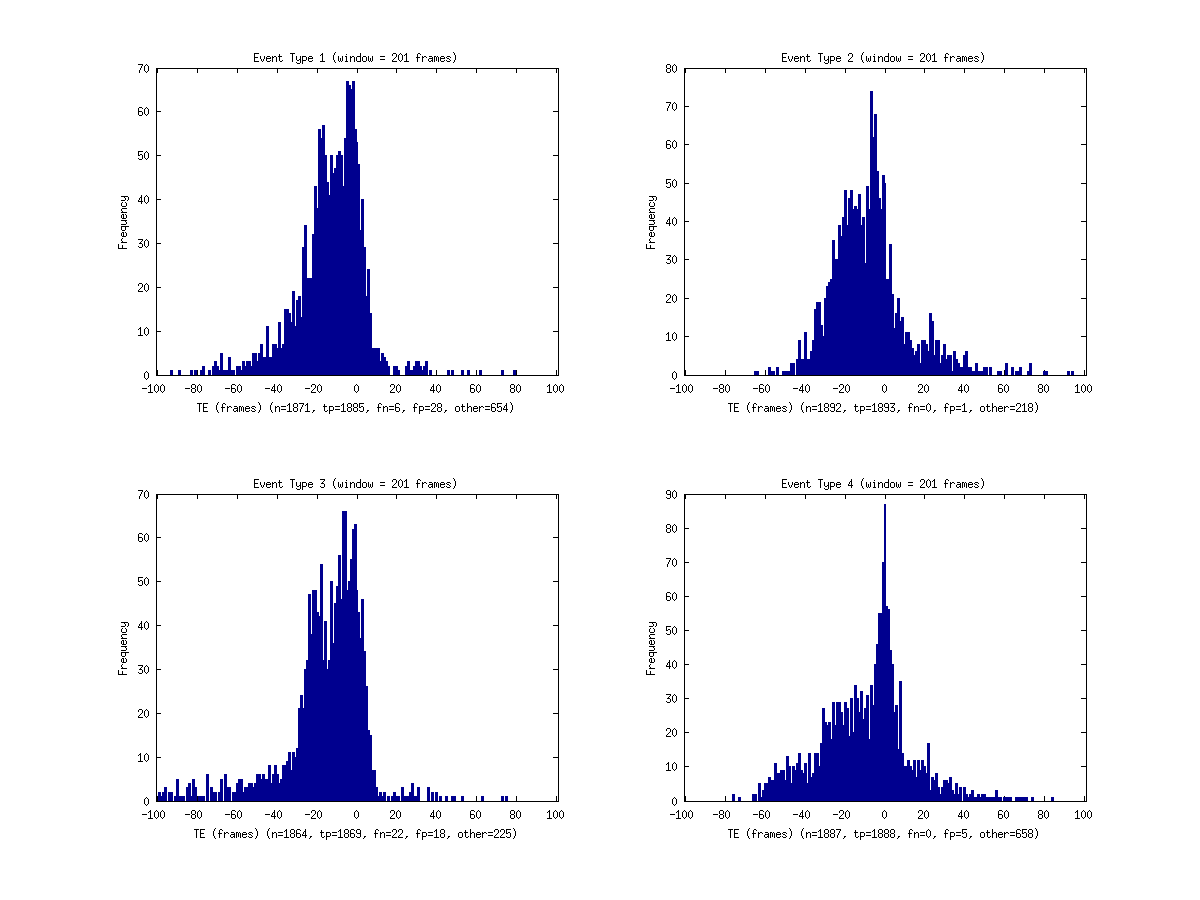
\includegraphics[width=0.70\textwidth]{figures/trueErrorsPerEventType_oconner.png}
\end{center}
\caption{
True errors per event type for O'Connor's heuristic. 
The data set consists of 8 subjects à 3 trials each.
The panes are (clockwise starting from the top-left):
Left Heel Strike, Right Toe Off, Right Heel Strike, Left Toe Off.
One frame corresponds to 1 ms.
If the estimated event was not within 100 frames from the true event then it is reported as "other" and not shown in the histogram.
}
\label{fig:oconner}
\end{figure*}

\begin{figure*}[t]
\begin{center}
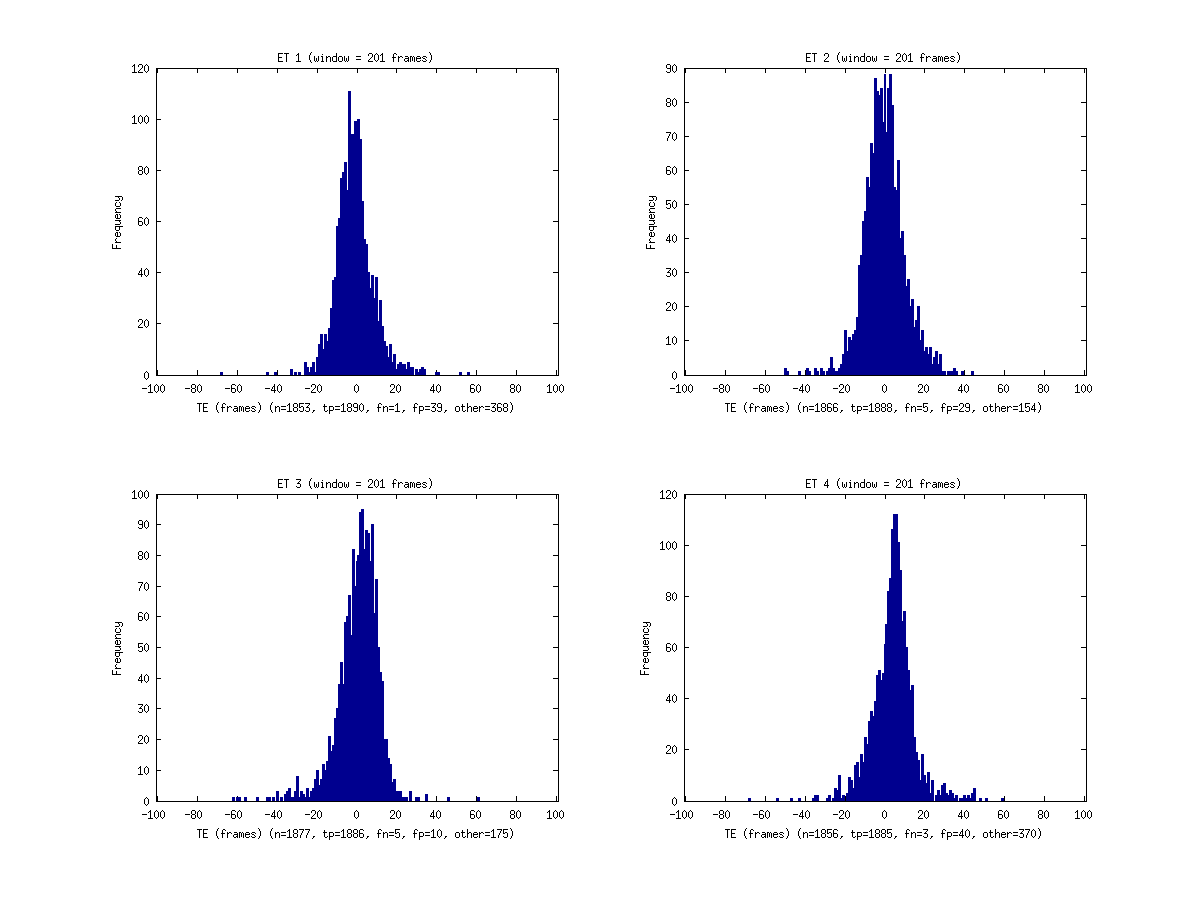
\includegraphics[width=0.70\textwidth]{figures/trueErrorsPerEventType_miller.png}
\end{center}
\caption{
True errors per event type for Miller's neural network.
The data set consists of 8 subjects à 3 trials each.
The panes are (clockwise starting from the top-left):
Left Heel Strike, Right Toe Off, Right Heel Strike, Left Toe Off.
One frame corresponds to 0.5 ms.
If the estimated event was not within 100 frames from the true event then it is reported as "other" and not shown in the histogram.
}
\label{fig:miller}
\end{figure*}

%\end{multicols}
\end{document}
